
\documentclass[twoside]{book}
\usepackage[]{graphicx}\usepackage[]{xcolor}
%% maxwidth is the original width if it is less than linewidth
%% otherwise use linewidth (to make sure the graphics do not exceed the margin)
\makeatletter
\def\maxwidth{ %
  \ifdim\Gin@nat@width>\linewidth
    \linewidth
  \else
    \Gin@nat@width
  \fi
}
\makeatother

\definecolor{fgcolor}{rgb}{0.345, 0.345, 0.345}
\newcommand{\hlnum}[1]{\textcolor[rgb]{0.686,0.059,0.569}{#1}}%
\newcommand{\hlstr}[1]{\textcolor[rgb]{0.192,0.494,0.8}{#1}}%
\newcommand{\hlcom}[1]{\textcolor[rgb]{0.678,0.584,0.686}{\textit{#1}}}%
\newcommand{\hlopt}[1]{\textcolor[rgb]{0,0,0}{#1}}%
\newcommand{\hlstd}[1]{\textcolor[rgb]{0.345,0.345,0.345}{#1}}%
\newcommand{\hlkwa}[1]{\textcolor[rgb]{0.161,0.373,0.58}{\textbf{#1}}}%
\newcommand{\hlkwb}[1]{\textcolor[rgb]{0.69,0.353,0.396}{#1}}%
\newcommand{\hlkwc}[1]{\textcolor[rgb]{0.333,0.667,0.333}{#1}}%
\newcommand{\hlkwd}[1]{\textcolor[rgb]{0.737,0.353,0.396}{\textbf{#1}}}%

\usepackage{framed}
\makeatletter
\newenvironment{kframe}{%
 \def\at@end@of@kframe{}%
 \ifinner\ifhmode%
  \def\at@end@of@kframe{\end{minipage}}%
  \begin{minipage}{\columnwidth}%
 \fi\fi%
 \def\FrameCommand##1{\hskip\@totalleftmargin \hskip-\fboxsep
 \colorbox{shadecolor}{##1}\hskip-\fboxsep
     % There is no \\@totalrightmargin, so:
     \hskip-\linewidth \hskip-\@totalleftmargin \hskip\columnwidth}%
 \MakeFramed {\advance\hsize-\width
   \@totalleftmargin\z@ \linewidth\hsize
   \@setminipage}}%
 {\par\unskip\endMakeFramed%
 \at@end@of@kframe}
\makeatother

\definecolor{shadecolor}{rgb}{.97, .97, .97}
\definecolor{messagecolor}{rgb}{0, 0, 0}
\definecolor{warningcolor}{rgb}{1, 0, 1}
\definecolor{errorcolor}{rgb}{1, 0, 0}
\newenvironment{knitrout}{}{} % an empty environment to be redefined in TeX

\usepackage{alltt}
\newcommand{\SweaveOpts}[1]{}  % do not interfere with LaTeX
\newcommand{\SweaveInput}[1]{} % because they are not real TeX commands
\newcommand{\Sexpr}[1]{}       % will only be parsed by R


\usepackage[margin=.9in]{geometry}
%\usepackage{kpfonts}   % for \varhearsuit
%\usepackage{txfonts}    % for \varhearsuit
\usepackage{amsmath}
\usepackage{probstat}
\usepackage{booktabs}
\def\Tri{\distribution{Triangle}}
\def\Rayleigh{\distribution{Rayleigh}}
\def\SD{\operatorname{SD}}
\usepackage{xstring}
\usepackage{makeidx}

%\def\Prob{\operatorname{Pr}}
\def\tnot{\operatorname{not}}
\usepackage{hyperref}
\usepackage{graphicx}
\usepackage{tikz}
\usetikzlibrary{patterns}
\usepackage[hidenotes]{authNote}
\usepackage[answerdelayed,exercisedelayed,lastexercise,chapter]{problems}

%\def\myindex#1{\relax}
%\def\Rindex#1{\relax}
\def\myindex#1{\index{#1}}

\usepackage{multicol}
\usepackage{longtable}
\renewcommand{\arraystretch}{1.4}

\def\sfrac#1#2{#1/#2}
\newcommand{\Partial}[2]{\frac{\partial #1}{\partial #2}}


\usepackage[Bjornstrup]{fncychap}
\usepackage{fancyhdr}
\pagestyle{fancy}
\fancyhf{}

%% Now begin customising things. See the fancyhdr docs for more info.

\renewcommand{\chaptermark}[1]{\thispagestyle{fancy}\markboth{{#1}}{}}
\renewcommand{\sectionmark}[1]{\markright{{#1}}{}}
%\renewcommand{\headrulewidth}{0pt}

\newcommand{\exampleidx}[1]{{\it #1}}
\newcommand{\defidx}[1]{{\bf #1}}
\newcommand{\mainidx}[1]{{\bf #1}}
\newcommand{\probidx}[1]{{{\underline{#1}}}}

\newcommand{\variable}[1]{{\color{green!50!black}\texttt{#1}}}
%\newcommand{\dataframe}[1]{{\color{blue!80!black}\texttt{#1}}}
%\newcommand{\Rindex}[2][black]{\index{{\color{#1}\texttt{#2}}}}
\newcommand{\Rindex}[1]{\index{\texttt{#1}}}
\newcommand{\dataframe}[1]{{\color{blue!80!black}\texttt{#1}}\Rindex{#1}}
\newcommand{\function}[1]{{\color{purple!75!blue}\texttt{\StrSubstitute{#1}{()}{}()}}\Rindex{#1}}
\newcommand{\option}[1]{{\color{brown!80!black}\texttt{#1}}}
\newcommand{\argument}[1]{{\color{brown!80!black}\texttt{#1}}}
%\newcommand{\pkg}[1]{{\color{red!80!black}\texttt{#1}}}
\newcommand{\pkg}[1]{{\color{red!80!black}\texttt{#1}}\Rindex{#1}}
\renewcommand{\code}[1]{{\color{blue!80!black}\texttt{#1}}}
% and for models
\newcommand{\model}[2]{{$\,$\hbox{#1}\ \ensuremath{\sim}\ \hbox{#2}}}

\DeclareSymbolFont{extraup}{U}{zavm}{m}{n}
\DeclareMathSymbol{\varheartsuit}{\mathalpha}{extraup}{86}
\DeclareMathSymbol{\vardiamondsuit}{\mathalpha}{extraup}{87}

\chead{}
\lhead[\sf \thepage]{\sf \leftmark}
\rhead[\sf \leftmark]{\sf \thepage}
\lhead[\sf \thepage]{\sf \thechapter. \leftmark}
\rhead[\sf \thechapter. \leftmark]{\sf \thepage}
\cfoot{}
\lfoot[\sf Last Modified: \today]{\sf Math 241 : Spring 2014 : Pruim}
\rfoot[\sf Math 241 : Spring 2014 : Pruim]{\sf Last Modified: \today}

\pagestyle{fancy}

\usepackage{sfsect}
\usepackage{relsize}

%%%%%%%%%%%%%%%%%%%%%%%%%%%%%%% macros %%%%%%%%%%%%%%%%%%%%%%%%%%%%%%%%%%%%%%%%%%

\def\Chapter#1{%
\chapter{#1}
%\setcounter{page}{1}%
}
\def\R{{\sf R}}
\def\Rstudio{{\sf RStudio}}
\def\term#1{\textbf{#1}}
\def\tab#1{{\sf #1}}


\newlength{\tempfmlength}
\newsavebox{\fmbox}
\newenvironment{fmpage}[1]
     {
	 \medskip
	 \setlength{\tempfmlength}{#1}
	 \begin{lrbox}{\fmbox}
	   \begin{minipage}{#1}
		 \vspace*{.02\tempfmlength}
		 \hfill
	   \begin{minipage}{.95 \tempfmlength}}
		 {\end{minipage}\hfill
		 \vspace*{.015\tempfmlength}
		 \end{minipage}\end{lrbox}\fbox{\usebox{\fmbox}}
	 \medskip
	 }


\newenvironment{boxedText}[1][.98\textwidth]%
{%
\begin{center}
\begin{fmpage}{#1}
}%
{%
\end{fmpage}
\end{center}
}

\newenvironment{boxedTable}[2][tbp]%
{%
\begin{table}[#1]
  \refstepcounter{table}
  \begin{center}
\begin{fmpage}{.98\textwidth}
  \begin{center}
	\sf \large Box~\expandafter\thetable. #2
\end{center}
\medskip
}%
{%
\end{fmpage}
\end{center}
\end{table}		% need to do something about exercises that follow boxedTable
}

\def\question{{\sf Q. }}
\def\answer{{\sf A. }}

\newcounter{example}[section]

\newenvironment{example}%
{\refstepcounter{example}%
\textbf{Example \thesection.\arabic{example}. }}%
{}

\newenvironment{examples}%
{\refstepcounter{example}%
\textbf{Examples \thesection.\arabic{example}. }}%
{}

\renewcommand{\theexample}{\thesection.\arabic{example}}



\newif\ifsolutions
\solutionstrue
\solutionsfalse

\newif\ifsolutionslocal
\solutionslocaltrue
\solutionslocalfalse

\parindent=0pt
\parskip=3mm



\begin{knitrout}
\definecolor{shadecolor}{rgb}{0.969, 0.969, 0.969}\color{fgcolor}\begin{kframe}


{\ttfamily\noindent\color{warningcolor}{\#\# Warning in library(package, lib.loc = lib.loc, character.only = TRUE, logical.return = TRUE, : there is no package called 'DAAG'}}

{\ttfamily\noindent\color{warningcolor}{\#\# Warning in library(package, lib.loc = lib.loc, character.only = TRUE, logical.return = TRUE, : there is no package called 'abd'}}

{\ttfamily\noindent\color{warningcolor}{\#\# Warning in library(package, lib.loc = lib.loc, character.only = TRUE, logical.return = TRUE, : there is no package called 'alr3'}}\end{kframe}
\end{knitrout}

%%%%%%%%%%%%%%%%%%%%%% title page info %%%%%%%%%%%%%%%%%%%%%%%%%%%%%%

\title{Math 241: Statistics for the Physical Sciences and Engineering}

\author{R Pruim}

\date{Spring 2014}

%%%%%%%%%%%%%%%%%%%%%%%%%%%%%%%%%%%%%%%%%%%%%%%%%%%%%%%%%%%%%%%%%%%%%
\makeindex
%%%%%%%%%%%%%%%%%%%%%%%%%%%%%%%%%%%%%%%%%%%%%%%%%%%%%%%%%%%%%%%%%%%%%

\lhead[\sf \thepage]{\sf \thechapter. \leftmark}
\rhead[\sf \thechapter. \leftmark]{\sf \thepage}



\begin{document}


\chapter{Linear Models}

In Chapter~\ref{chap:propagation} we learned how to estimate one quantity based
on its (known) relationship to other quantities.  For example, we estimated the
number of dimes in a sack of dimes from our estimates of the weight of the
dimes and the average weight of a dime.  

In this chapter we will explore how to use data to determine the relationship among
two or more variables when this relationship is not know in advance.  The general
framework we will use is 

\[
Y = f(x_1, x_2, \dots, x_k) + \varepsilon
\]
\begin{itemize}
	\item $Y$ is the \term{response} variable that we are trying to estimate
		from $k$ \term{explanatory} variables $x_1, x_2, \dots, x_k$.
	\item
		The relationship between the explanatory variables and the response 
		variables is described by a function $f$.
	\item
		The relationship described by $f$ need not be a perfect fit.  The \term{error}
		term in the model, $\varepsilon$, describes how individual responses
		differ from the value give by $f$.  
		
		We will model $\varepsilon$ with a 
		distribution -- typically a distribution with a mean of 0 -- 
		so another way to think about this model is the for a given 
		values of the predictors, the values of $Y$ have a distribution.  The mean
		of this distribution is specified by $f$ and the shape by $\varepsilon$.
\end{itemize}


\section{The Simple Linear Regression Model}

\[
Y = \beta_0 + \beta_1 x + \varepsilon  \qquad \mbox{where $\varepsilon \sim \Norm(0,\sigma)$.}
\]

In other words:
\begin{itemize}
\item
The mean response for a given predictor value $x$ is given by a linear formula
\[
\mbox{mean response} = \beta_0 + \beta_1 x
\]
This can also be written as 
\[
\E(Y \mid X=x) = \beta_0 + \beta_1 x)
\]
\item
The distribution of all responses for a given predictor value $x$ is normal.
\item
The standard deviation of the responses is the same for each predictor value,
\end{itemize}
Furthermore, in this model the values of $\varepsilon$ are independent.

There are many different things we might want to do with a linear model, for example:
\begin{itemize}
	\item Estimate the coefficients $\beta_0$ and $\beta_1$.
	\item Estimate the value $Y$ associated with a particular value of $x$.
	\item Say something about how well a line fits the data.
\end{itemize}

\section{Fitting the Simple Linear Model}

\subsection{The Least Squares Method}

We want to determine the best fitting line to the data.  The usual method is 
the method of least squares\footnote{In this case, it turns out that the least 
squares and maximum likelihood methods produce exactly the same results.}
which chooses the line that has the 
\emph{ smallest possible sum of squares of residuals}, where residuals are defined by

\[
\mbox{residual} = \mbox{observed} - \mbox{predicted}
\]

\begin{example}
Consider the following small data set.
\begin{multicols}{2}
\begin{knitrout}
\definecolor{shadecolor}{rgb}{0.969, 0.969, 0.969}\color{fgcolor}\begin{kframe}
\begin{alltt}
\hlstd{someData} \hlkwb{<-} \hlkwd{data.frame}\hlstd{(}
  \hlkwc{x}\hlstd{=}\hlnum{1}\hlopt{:}\hlnum{5}\hlstd{,}
  \hlkwc{y}\hlstd{=}\hlkwd{c}\hlstd{(}\hlnum{1}\hlstd{,}\hlnum{3}\hlstd{,}\hlnum{2}\hlstd{,}\hlnum{4}\hlstd{,}\hlnum{4}\hlstd{)}
\hlstd{)}
\hlstd{someData}
\end{alltt}
\begin{verbatim}
##   x y
## 1 1 1
## 2 2 3
## 3 3 2
## 4 4 4
## 5 5 4
\end{verbatim}
\end{kframe}
\end{knitrout}
\begin{knitrout}
\definecolor{shadecolor}{rgb}{0.969, 0.969, 0.969}\color{fgcolor}\begin{kframe}
\begin{alltt}
\hlkwd{xyplot}\hlstd{( y} \hlopt{~} \hlstd{x,}
  \hlkwc{data}\hlstd{=someData,} \hlkwc{type}\hlstd{=}\hlkwd{c}\hlstd{(}\hlstr{'p'}\hlstd{,}\hlstr{'g'}\hlstd{),}
  \hlkwc{ylim}\hlstd{=}\hlkwd{c}\hlstd{(}\hlnum{0}\hlstd{,}\hlnum{5}\hlstd{),} \hlkwc{xlim}\hlstd{=}\hlkwd{c}\hlstd{(}\hlnum{0}\hlstd{,}\hlnum{6}\hlstd{))}
\end{alltt}
\end{kframe}

{\centering 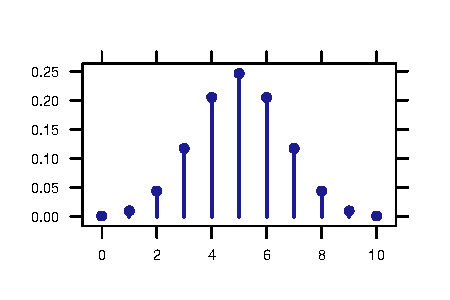
\includegraphics[width=\maxwidth]{figures/fig-unnamed-chunk-2-1} 

}



\end{knitrout}
\end{multicols}

\begin{enumerate}
	\item
		Add a line to the plot that ``fits the data well".  Don't do any calculations,
		just add the line.
	\item
		Now estimate the residuals for each point relative to your line
	\item
		Compute the sum of the squared residuals, $SSE$.
	\item
		Estimate the slope and intercept of your line.
\end{enumerate}

\newpage
For example, suppose we we select a line that passes through $(0,1)$ and $(5,4)$. 
the equation for this line is $y = 1 + .6 x$, and it looks like a pretty good fit:
\begin{knitrout}
\definecolor{shadecolor}{rgb}{0.969, 0.969, 0.969}\color{fgcolor}\begin{kframe}
\begin{alltt}
\hlkwd{xyplot}\hlstd{(y} \hlopt{~} \hlstd{x,} \hlkwc{data} \hlstd{= someData,} \hlkwc{xlim} \hlstd{=} \hlkwd{c}\hlstd{(}\hlnum{0}\hlstd{,} \hlnum{6}\hlstd{),} \hlkwc{ylim} \hlstd{=} \hlkwd{c}\hlstd{(}\hlnum{0}\hlstd{,} \hlnum{5}\hlstd{))}
\hlstd{f} \hlkwb{<-} \hlkwd{makeFun}\hlstd{(}\hlnum{1} \hlopt{+} \hlnum{0.6} \hlopt{*} \hlstd{x} \hlopt{~} \hlstd{x)}
\hlkwd{plotFun}\hlstd{(}\hlkwd{f}\hlstd{(x)} \hlopt{~} \hlstd{x,} \hlkwc{add} \hlstd{=} \hlnum{TRUE}\hlstd{,} \hlkwc{col} \hlstd{=} \hlstr{"gray50"}\hlstd{)}
\end{alltt}
\end{kframe}

{\centering 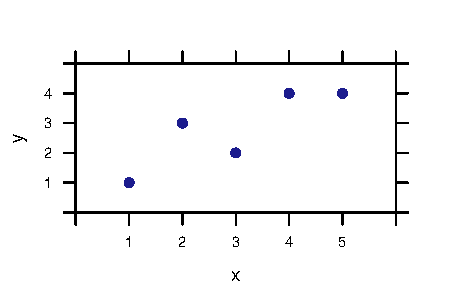
\includegraphics[width=\maxwidth]{figures/fig-unnamed-chunk-3-1} 
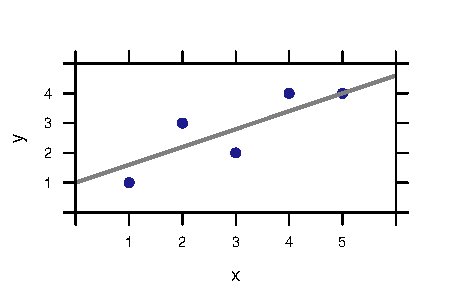
\includegraphics[width=\maxwidth]{figures/fig-unnamed-chunk-3-2} 

}



\end{knitrout}
The residuals for this function are 
\begin{knitrout}
\definecolor{shadecolor}{rgb}{0.969, 0.969, 0.969}\color{fgcolor}\begin{kframe}
\begin{alltt}
\hlstd{resids} \hlkwb{<-} \hlkwd{with}\hlstd{(someData, y} \hlopt{-} \hlkwd{f}\hlstd{(x)) ; resids}
\end{alltt}
\begin{verbatim}
## [1] -0.6  0.8 -0.8  0.6  0.0
\end{verbatim}
\end{kframe}
\end{knitrout}
and $SSE$ is 
\begin{knitrout}
\definecolor{shadecolor}{rgb}{0.969, 0.969, 0.969}\color{fgcolor}\begin{kframe}
\begin{alltt}
\hlkwd{sum}\hlstd{(resids}\hlopt{^}\hlnum{2}\hlstd{)}
\end{alltt}
\begin{verbatim}
## [1] 2
\end{verbatim}
\end{kframe}
\end{knitrout}
If your line is a good fit, then $SSE$ will be small.  
The best fitting line will have the smallest possible $SSE$.   
The \function{lm()} function will find this best fitting line for us.
\begin{knitrout}
\definecolor{shadecolor}{rgb}{0.969, 0.969, 0.969}\color{fgcolor}\begin{kframe}
\begin{alltt}
\hlstd{model1} \hlkwb{<-} \hlkwd{lm}\hlstd{( y} \hlopt{~} \hlstd{x,} \hlkwc{data}\hlstd{=someData ); model1}
\end{alltt}
\begin{verbatim}
## 
## Call:
## lm(formula = y ~ x, data = someData)
## 
## Coefficients:
## (Intercept)            x  
##         0.7          0.7
\end{verbatim}
\end{kframe}
\end{knitrout}
This says that the equation of the best fit line is 
\[
\hat y = 0.7 + 0.7 x
\]

\begin{knitrout}
\definecolor{shadecolor}{rgb}{0.969, 0.969, 0.969}\color{fgcolor}\begin{kframe}
\begin{alltt}
\hlkwd{xyplot}\hlstd{(y} \hlopt{~} \hlstd{x,} \hlkwc{data} \hlstd{= someData,} \hlkwc{type} \hlstd{=} \hlkwd{c}\hlstd{(}\hlstr{"p"}\hlstd{,} \hlstr{"r"}\hlstd{))}
\end{alltt}
\end{kframe}

{\centering 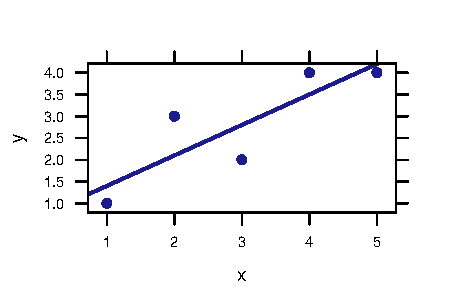
\includegraphics[width=\maxwidth]{figures/fig-unnamed-chunk-7-1} 

}



\end{knitrout}
We can compute $SSE$ using the \function{resid()} function.
\begin{knitrout}
\definecolor{shadecolor}{rgb}{0.969, 0.969, 0.969}\color{fgcolor}\begin{kframe}
\begin{alltt}
\hlstd{SSE} \hlkwb{<-} \hlkwd{sum} \hlstd{(} \hlkwd{resid}\hlstd{(model1)}\hlopt{^}\hlnum{2} \hlstd{); SSE}
\end{alltt}
\begin{verbatim}
## [1] 1.9
\end{verbatim}
\end{kframe}
\end{knitrout}
As we see, this is a better fit than our first attempt -- 
at least according to the least squares criterion.
It will better than \emph{any} other attempt -- it is the least 
squares regression line.
\end{example}

\subsection{Properties of the Least Squares Regression Line}
For a line with equation $y = \hat\beta_0 + \hat\beta_1 x$, the residuals are 
\[
e_i = y_i - (\hat\beta_0 + \hat\beta_1 x) 
\]
and the sum of the squares of the residuals is 
\[
SSE = \sum e_i^2  = \sum (y_i - (\hat\beta_0 + \hat\beta_1 x) )^2
\]
Simple calculus (which we won't do here) allows us to compute the 
best $\hat\beta_0$ and $\hat\beta_1$ possible.  
These best values define the least squares regression line.
We always compute these values using software, but it is good to note that 
the least squares line satisfies two very nice properties.
\begin{enumerate}
\item
The point $(\mean x, \mean y)$ is on the line. 

This means that $\mean y = \hat\beta_0 + \hat\beta_1 \mean x$  (and $\hat\beta_0 = \mean y - \hat\beta_1 \mean x$)
\item
The slope of the line is $\displaystyle b = r \frac{s_y}{s_x}$ where $r$ is the 
\term{correlation coefficient}:
\myindex{correlation coefficient}%
\[
r = \frac{1}{n-1} \sum \frac{ x_i - \mean x }{s_x} \cdot \frac{ y_i - \mean y }{s_y}
\]
\end{enumerate}
Since we have a point and the slope, it is easy to compute the equation for the line
if we know $\mean x$, $s_x$, $\mean y$, $s_y$, and $r$.

\subsection{An Example: Estimating OSA}
\begin{example}
In a study of eye strain caused by visual display terminals, researchers wanted
to be able to estimate ocular surface area (OSA) from palpebral fissure (the
horizontal width of the eye opening in cm) because palpebral fissue is easier
to measure than OSA.
\begin{knitrout}
\definecolor{shadecolor}{rgb}{0.969, 0.969, 0.969}\color{fgcolor}\begin{kframe}
\begin{alltt}
\hlcom{# require(Devore6) #this package no longer updated on CRAN (checked 27 jan 2015) -- will it}
\hlcom{# work with v7 (Devore7 package)??  NO...so have to use old version if you want to use}
\hlcom{# these data...}
\hlkwd{require}\hlstd{(Devore6)}
\hlkwd{head}\hlstd{(xmp12.01,} \hlnum{3}\hlstd{)}
\end{alltt}
\begin{verbatim}
##   palprebal  OSA
## 1      0.40 1.02
## 2      0.42 1.21
## 3      0.48 0.88
\end{verbatim}
\begin{alltt}
\hlcom{# note misspelling in this data set; let's fix it}
\hlkwd{names}\hlstd{(xmp12.01)[}\hlnum{1}\hlstd{]} \hlkwb{<-} \hlstr{"palpebral"}
\hlkwd{names}\hlstd{(xmp12.01)}
\end{alltt}
\begin{verbatim}
## [1] "palpebral" "OSA"
\end{verbatim}
\begin{alltt}
\hlstd{x.bar} \hlkwb{<-} \hlkwd{mean}\hlstd{(}\hlopt{~}\hlstd{palpebral,} \hlkwc{data} \hlstd{= xmp12.01)}
\hlstd{y.bar} \hlkwb{<-} \hlkwd{mean}\hlstd{(}\hlopt{~}\hlstd{OSA,} \hlkwc{data} \hlstd{= xmp12.01)}
\hlstd{s_x} \hlkwb{<-} \hlkwd{sd}\hlstd{(}\hlopt{~}\hlstd{palpebral,} \hlkwc{data} \hlstd{= xmp12.01)}
\hlstd{s_y} \hlkwb{<-} \hlkwd{sd}\hlstd{(}\hlopt{~}\hlstd{OSA,} \hlkwc{data} \hlstd{= xmp12.01)}
\hlstd{r} \hlkwb{<-} \hlkwd{cor}\hlstd{(xmp12.01}\hlopt{$}\hlstd{palpebral, xmp12.01}\hlopt{$}\hlstd{OSA)}
\hlkwd{c}\hlstd{(}\hlkwc{x.bar} \hlstd{= x.bar,} \hlkwc{y.bar} \hlstd{= y.bar,} \hlkwc{s_x} \hlstd{= s_x,} \hlkwc{s_y} \hlstd{= s_y,} \hlkwc{r} \hlstd{= r)}
\end{alltt}
\begin{verbatim}
##     x.bar     y.bar       s_x       s_y         r 
## 1.0513333 2.8403333 0.3798160 1.2083374 0.9681245
\end{verbatim}
\begin{alltt}
\hlstd{slope} \hlkwb{<-} \hlstd{r} \hlopt{*} \hlstd{s_y}\hlopt{/}\hlstd{s_x}
\hlstd{intercept} \hlkwb{<-} \hlstd{y.bar} \hlopt{-} \hlstd{slope} \hlopt{*} \hlstd{x.bar}
\hlkwd{c}\hlstd{(}\hlkwc{intercept} \hlstd{= intercept,} \hlkwc{slope} \hlstd{= slope)}
\end{alltt}
\begin{verbatim}
##  intercept      slope 
## -0.3977389  3.0799672
\end{verbatim}
\end{kframe}
\end{knitrout}
\end{example}

Fortunately, statistical software packages do all this work for us, so the
caclulations of the preceding example don't need to be done in practice.

\begin{example}
In a study of eye strain caused by visual display terminals, researchers wanted
to be able to estimate ocular surface area (OSA) from palpebral fissure (the
horizontal width of the eye opening in cm) because palpebral fissue is easier
to measure than OSA.
\begin{knitrout}
\definecolor{shadecolor}{rgb}{0.969, 0.969, 0.969}\color{fgcolor}\begin{kframe}
\begin{alltt}
\hlstd{osa.model} \hlkwb{<-} \hlkwd{lm}\hlstd{(OSA} \hlopt{~} \hlstd{palpebral,} \hlkwc{data} \hlstd{= xmp12.01)}
\hlstd{osa.model}
\end{alltt}
\begin{verbatim}
## 
## Call:
## lm(formula = OSA ~ palpebral, data = xmp12.01)
## 
## Coefficients:
## (Intercept)    palpebral  
##     -0.3977       3.0800
\end{verbatim}
\end{kframe}
\end{knitrout}
\function{lm()} stands for linear model.  The default output includes the estimates
of the coefficients ($\hat\beta_0$ and $\hat \beta_1$) based on the data.  If that is the 
only information we want, then we can use 
\begin{knitrout}
\definecolor{shadecolor}{rgb}{0.969, 0.969, 0.969}\color{fgcolor}\begin{kframe}
\begin{alltt}
\hlkwd{coef}\hlstd{(osa.model)}
\end{alltt}
\begin{verbatim}
## (Intercept)   palpebral 
##  -0.3977389   3.0799672
\end{verbatim}
\end{kframe}
\end{knitrout}

This means that the equation of the least squares regression line is 
\[
\hat y = \ensuremath{-0.398} + 3.08 x
\]

We use $\hat y$ to indicate that this is not an observed value of the response variable
but an estimated value (based on the linear equation given).

\R\ can add a regression line to our scatter plot if we ask it to.
\begin{center}
\begin{knitrout}
\definecolor{shadecolor}{rgb}{0.969, 0.969, 0.969}\color{fgcolor}\begin{kframe}
\begin{alltt}
\hlkwd{xyplot}\hlstd{(OSA} \hlopt{~} \hlstd{palpebral,} \hlkwc{data} \hlstd{= xmp12.01,} \hlkwc{type} \hlstd{=} \hlkwd{c}\hlstd{(}\hlstr{"p"}\hlstd{,} \hlstr{"r"}\hlstd{))}
\end{alltt}
\end{kframe}

{\centering 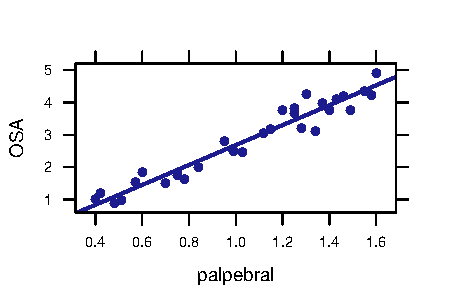
\includegraphics[width=\maxwidth]{figures/fig-osa-scatter-1} 

}



\end{knitrout}
\end{center}

We see that the line does run roughly ``through the middle'' of the dat but that
there is some variability above and below the line.
\end{example}

\subsection{Explanatory and Response Variables Matter}
It is important that 
the explanatory variable be the ``\variable{x}'' variable
and the response variable be the ``\variable{y}'' variable
when doing regression.  If we reverse the roles of \variable{OSA} and 
\variable{palpebral}
we do not get the same model.  This is because the residuals are measured vertically 
(in the $y$ direction).  


\section{Estimating the Response}

We can use our least squares regression line to estimate the value of the response
variable from the value of the explanatory variable.

\begin{example}
If the palpebral width is 1.2 cm, then we would estimate OSA to be 

\[
\hat{\texttt{osa}} = 
\ensuremath{-0.398} + 3.08 \cdot 1.2 
= 3.298 
\]

\R\ can automate this for us too.  The \function{makeFun()} function will
create a function from our model.  
If we input a palpebral measurement into this function, the function
will return the estimated OSA.
\begin{knitrout}
\definecolor{shadecolor}{rgb}{0.969, 0.969, 0.969}\color{fgcolor}\begin{kframe}
\begin{alltt}
\hlstd{estimated.osa} \hlkwb{<-} \hlkwd{makeFun}\hlstd{(osa.model)}
\hlkwd{estimated.osa}\hlstd{(}\hlnum{1.2}\hlstd{)}
\end{alltt}
\begin{verbatim}
##        1 
## 3.298222
\end{verbatim}
\end{kframe}
\end{knitrout}

As it turns out, the 17th measurement in our data set had a
\variable{palpebral} measurement of 1.2 cm.
\begin{knitrout}
\definecolor{shadecolor}{rgb}{0.969, 0.969, 0.969}\color{fgcolor}\begin{kframe}
\begin{alltt}
\hlstd{xmp12.01[}\hlnum{17}\hlstd{, ]}
\end{alltt}
\begin{verbatim}
##    palpebral  OSA
## 17       1.2 3.76
\end{verbatim}
\end{kframe}
\end{knitrout}
The corresponding OSA of 3.76 means that the residual for this observation is 
\[
\mbox{observed} - \mbox{predicted} = 3.76 - 3.2982218 = 
0.4617782  
\]
\end{example}

\section{Parameter Estimates}
\subsection{Interpreting the Coefficients}
The coefficients of the linear model tell us how to construct the linear function
that we use to estimate response values, but they can be interesting in their own
rite as well.

The intercept $\beta_0$ is the mean response value when the 
explanatory variable is 0.  This may or may not be interesting.
Often $\beta_0$ is not interesting because we are not interested
in the value of the response variable when the predictor is 0.  (That might not 
even be a possible value for the predictor.)  Furthermore, 
if we do not collect data with values of the explanatory variable near 0, then
we will be extrapolating from our data when we talk about the intercept.

The estimate for $\beta_1$, on the other hand, is nearly always of interest.
The slope coefficient $\beta_1$ tells us how quickly the response variable changes 
per unit change in the predictor.  This is an interesting value in many more situations.
Furthermore, when $\beta_1 = 0$, then our model does not depend on the predictor at all.
So when 0 is contained in the confidence interval for $\beta_1$, we do not have sufficient 
evidence to be convinced that our predictor is of any use in predicting the response.

\subsection{Estimating $\sigma$}

There is one more parameter in our model that we have been mostly ignoring so far: $\sigma$ (or 
equivalently $\sigma^2$).  This is the parameter that describes how tightly things should 
cluster around the regression line.  We can estimate $\sigma^2$ from our residuals:

\begin{align*}
\hat\sigma^2 & = MSE = \frac{ \sum_i e_i^2 }{ n -2 }
\\
\hat\sigma & = RMSE = \sqrt{MSE} = \sqrt{\frac{ \sum_i e_i^2 }{ n -2 } }
\end{align*}
The acronyms $MSE$ and $RMSE$ stand for \term{Mean Squared Error} and 
\term{Root Mean Squared Error}.
The numerator in these expressions is the sum of the squares of the residuals
\[
SSE = \sum_i e_i^2 \;.
\]
This is precisely the quantity that we were minimizing to get our least squares fit.
\[
MSE = \frac{SSE}{DFE} 
\]
where $DFE = n-2$ is the \term{degrees of freedom} associated with the
estimation of $\sigma^2$ in a simple linear model.  We lose two degrees of
freedom when we estimate $\beta_0$ and $\beta_1$, just like we lost 1 degree of
freedom when we had to estimate $\mu$ in order to compute a sample variance.

$RMSE = \sqrt{MSE}$ is listed in the summary output for the linear model as the
\term{residual standard error} because it is the estimated standard deviation of 
the error terms in the model.
\begin{knitrout}
\definecolor{shadecolor}{rgb}{0.969, 0.969, 0.969}\color{fgcolor}\begin{kframe}
\begin{alltt}
\hlkwd{summary}\hlstd{(osa.model)}
\end{alltt}
\begin{verbatim}
## 
## Call:
## lm(formula = OSA ~ palpebral, data = xmp12.01)
## 
## Residuals:
##      Min       1Q   Median       3Q      Max 
## -0.60942 -0.19875 -0.01902  0.21727  0.66378 
## 
## Coefficients:
##             Estimate Std. Error t value Pr(>|t|)
## (Intercept)  -0.3977     0.1680  -2.367   0.0251
## palpebral     3.0800     0.1506  20.453   <2e-16
## 
## Residual standard error: 0.308 on 28 degrees of freedom
## Multiple R-squared:  0.9373,	Adjusted R-squared:  0.935 
## F-statistic: 418.3 on 1 and 28 DF,  p-value: < 2.2e-16
\end{verbatim}
\end{kframe}
\end{knitrout}
We will learn about other parts of this summary output shortly.
Much is known about the estimator $\sigma^2$, including 
\begin{itemize}
	\item $\hat \sigma^2$ is unbiased (on average it is $\sigma^2$), and 
	\item
		the sampling distribution is a Chi-Squared distribution with
		$n-2$ degrees of freedom.  
		(Chi-Squared distributions are a special case of Gamma distributions.)
\end{itemize}


\section{Checking Assumptions}

\subsection{Don't Fit a Line If a Line Doesn't Fit}

The least squares method can be used to fit a line to any data -- even if a line
is not a useful representation of the relationship between the variables.
When doing regression we should always look at the data to see if a line 
is a good fit.  If it is not, then the simple linear model is not a good choice and 
we should look for some other model that does a better job of describing the 
relationship between our two variables.  

\subsection{Checking the Residuals}

Residuals should also be checked to see that the distribution looks approximately
normal and that that standard deviation remains consistent across the range of
our data (and across time).
Often it is easier to asses the linear fit by looking at a plot of the 
residuals than by looking at the natural scatter plot because on the scale 
of the residuals, discrepancies are easier to see.

\begin{example}
Returning to our OSA data, we can make plots of all the residuals using the 
\function{resid()} function.
\begin{knitrout}
\definecolor{shadecolor}{rgb}{0.969, 0.969, 0.969}\color{fgcolor}\begin{kframe}
\begin{alltt}
\hlkwd{xyplot}\hlstd{(}\hlkwd{resid}\hlstd{(osa.model)} \hlopt{~} \hlstd{palpebral,} \hlkwc{data} \hlstd{= xmp12.01)}
\hlkwd{qqmath}\hlstd{(}\hlopt{~}\hlkwd{resid}\hlstd{(osa.model),} \hlkwc{data} \hlstd{= xmp12.01)}
\end{alltt}
\end{kframe}

{\centering 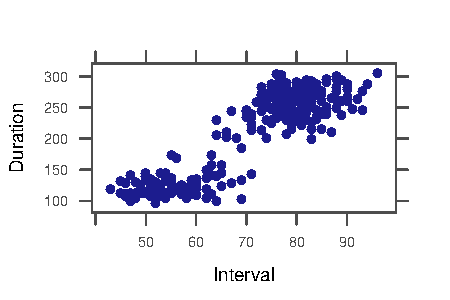
\includegraphics[width=\maxwidth]{figures/fig-unnamed-chunk-15-1} 
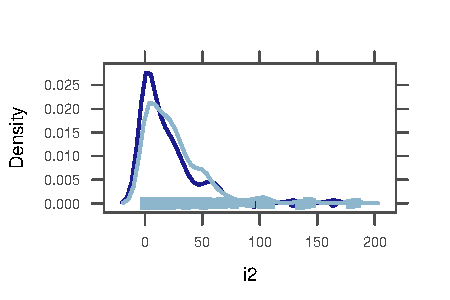
\includegraphics[width=\maxwidth]{figures/fig-unnamed-chunk-15-2} 

}



\end{knitrout}
\end{example}
If the assumptions of the model are correct, there should be no distinct patterns to this scatter
plot (usually called a residual plot) and the normal-quantile plot should be roughly linear
since the model says that differences between observed responses and the true linear fit
should be random noise following a normal distribution with constant standard deviation.

In this case things look pretty good. 

\subsection{Outliers in Regression}

Outliers can be very influential in regression, especially in small data sets,
and especially if they occur for extreme values of the explanatory variable.
Outliers cannot be removed just because we don't like them, but they should be
explored to see what is going on (data entry error? special case? etc.)

Some researchers will do ``leave-one-out'' analysis, or ``leave some out'' analysis
where they refit the regression with each data point left out once.  If the regression
summary changes very little when we do this, this means that the regression line
is summarizing information that is shared among all the points relatively equally.
But if removing one or a small number of values makes a dramatic change, then
we know that that point is exerting a lot of influence over the resulting
analysis (a cause for caution).   

\section{How Good Are Our Estimates?}
Assuming our diagnostics indicate that fitting a linear model is reasonable for our data,
our next question is \emph{How good are our estimates?}
Notice that there are several things we have estimated:
\begin{itemize}
	\item The intercept coefficient $\beta_0$ 
		[estimate: $\hat \beta_0$]
	\item The slope coefficient $\beta_1$ 
		[estimate: $\hat \beta_1$]
	\item Values of $y$ for given values of $x$. 
		[estimate: $\hat y = \hat \beta_0 + \hat \beta_1 x$]
\end{itemize}

We would like to be able to compute uncertainties and confidence intervals for these.
Fortunately, \R\ makes this straightforward.

\subsection{Estimating the $\beta$s}

\begin{example}
	\question
	Returning to the OSA data, compute standard uncertainties and 95\% confidence intervals
	for $\beta_0$ and $\beta_1$.

	\answer
	The \function{summary()} function provides additional information about the 
	model:
\begin{knitrout}
\definecolor{shadecolor}{rgb}{0.969, 0.969, 0.969}\color{fgcolor}\begin{kframe}
\begin{alltt}
\hlkwd{summary}\hlstd{(osa.model)}
\end{alltt}
\begin{verbatim}
## 
## Call:
## lm(formula = OSA ~ palpebral, data = xmp12.01)
## 
## Residuals:
##      Min       1Q   Median       3Q      Max 
## -0.60942 -0.19875 -0.01902  0.21727  0.66378 
## 
## Coefficients:
##             Estimate Std. Error t value Pr(>|t|)
## (Intercept)  -0.3977     0.1680  -2.367   0.0251
## palpebral     3.0800     0.1506  20.453   <2e-16
## 
## Residual standard error: 0.308 on 28 degrees of freedom
## Multiple R-squared:  0.9373,	Adjusted R-squared:  0.935 
## F-statistic: 418.3 on 1 and 28 DF,  p-value: < 2.2e-16
\end{verbatim}
\end{kframe}
\end{knitrout}
	We don't know what to do with all of the information displayed here, but we can see
	some familiar things in the coefficient table.  
If we only want the coefficients part of the summary output we can get that using
\begin{knitrout}
\definecolor{shadecolor}{rgb}{0.969, 0.969, 0.969}\color{fgcolor}\begin{kframe}
\begin{alltt}
\hlkwd{coef}\hlstd{(}\hlkwd{summary}\hlstd{(osa.model))}
\end{alltt}
\begin{verbatim}
##               Estimate Std. Error   t value     Pr(>|t|)
## (Intercept) -0.3977389  0.1680090 -2.367367 2.506081e-02
## palpebral    3.0799672  0.1505882 20.452918 2.252825e-18
\end{verbatim}
\end{kframe}
\end{knitrout}
	From this we see the estimates ($\hat \beta$'s)
	displayed again.  Next to each of those is a standard error.  That is the standard
	uncertainty for these estimates.  So we could report our estimated coefficients as 
	\[
	\beta_0: -0.40 \pm 
		0.17
	\qquad
	\beta_1: 3.08 \pm 
		0.15
	\]

	A confidence interval can be computed using
	\[
	\hat\beta_i \pm t_* SE_{\beta_i}
	\]
	because 
	\begin{itemize}
		\item
	the sampling distribution for $\hat \beta_i$ 
			is normal, 
		\item
	the sampling distribution for $\hat \beta_i$ 
			is unbiased (the mean is $\beta_i$), and
		\item
			the standard deviation of the sampling distribution depends on $\sigma$ 
			(and some other things), but
		\item
			we don't know $\sigma$, so we have to estimate it using $RMSE = \sqrt{MSE}$.
	\end{itemize}

\begin{knitrout}
\definecolor{shadecolor}{rgb}{0.969, 0.969, 0.969}\color{fgcolor}\begin{kframe}
\begin{alltt}
\hlstd{t.star} \hlkwb{<-} \hlkwd{qt}\hlstd{(}\hlnum{.975}\hlstd{,} \hlkwc{df}\hlstd{=}\hlnum{28}\hlstd{); t.star}    \hlcom{# n-2 degrees of freedom for simple linear regression}
\end{alltt}
\begin{verbatim}
## [1] 2.048407
\end{verbatim}
\begin{alltt}
\hlstd{t.star} \hlopt{*} \hlnum{0.151}
\end{alltt}
\begin{verbatim}
## [1] 0.3093095
\end{verbatim}
\end{kframe}
\end{knitrout}
	So a 95\% confidence interval for $\beta_1$ is 
	\[
	3.08 \pm 0.31
	\]
	The degrees of freedom used are $DFE = n-2$, the same as used in the estimate of $\sigma^2$.
	(We are using a t-distribution instead of a normal distribution because we don't know 
	$\sigma$.  The degrees of freedom are those associated with using $RMSE = \sqrt{MSE}$
	as our estimate for $\sigma$.)

	\R\ can compute confidence intervals for both parameters using the function
	\function{confint()}:
\begin{knitrout}
\definecolor{shadecolor}{rgb}{0.969, 0.969, 0.969}\color{fgcolor}\begin{kframe}
\begin{alltt}
\hlkwd{confint}\hlstd{(osa.model)}
\end{alltt}
\begin{verbatim}
##                  2.5 %      97.5 %
## (Intercept) -0.7418897 -0.05358811
## palpebral    2.7715014  3.38843310
\end{verbatim}
\end{kframe}
\end{knitrout}
A 68\% confidence interval should have a margin of error of approximately 1 standard
uncertainty:
\begin{knitrout}
\definecolor{shadecolor}{rgb}{0.969, 0.969, 0.969}\color{fgcolor}\begin{kframe}
\begin{alltt}
\hlkwd{confint}\hlstd{(osa.model,} \hlkwc{level} \hlstd{=} \hlnum{0.68}\hlstd{)}
\end{alltt}
\begin{verbatim}
##                   16 %       84 %
## (Intercept) -0.5678369 -0.2276409
## palpebral    2.9275067  3.2324278
\end{verbatim}
\begin{alltt}
\hlkwd{apply}\hlstd{(}\hlkwd{confint}\hlstd{(osa.model,} \hlkwc{level} \hlstd{=} \hlnum{0.68}\hlstd{),} \hlnum{1}\hlstd{, diff)}\hlopt{/}\hlnum{2}  \hlcom{# half width of CIs}
\end{alltt}
\begin{verbatim}
## (Intercept)   palpebral 
##   0.1700980   0.1524606
\end{verbatim}
\end{kframe}
\end{knitrout}

\end{example}

\subsection{Confidence and Prediction Intervals for the Response Value}
We can also create interval estimates for the response.    \R\ will compute
this if we simply ask:
\begin{knitrout}
\definecolor{shadecolor}{rgb}{0.969, 0.969, 0.969}\color{fgcolor}\begin{kframe}
\begin{alltt}
\hlstd{estimated.osa} \hlkwb{<-} \hlkwd{makeFun}\hlstd{(osa.model)}
\hlkwd{estimated.osa}\hlstd{(}\hlnum{1.2}\hlstd{,} \hlkwc{interval} \hlstd{=} \hlstr{"confidence"}\hlstd{)}
\end{alltt}
\begin{verbatim}
##        fit      lwr      upr
## 1 3.298222 3.174238 3.422206
\end{verbatim}
\begin{alltt}
\hlkwd{estimated.osa}\hlstd{(}\hlnum{0.8}\hlstd{,} \hlkwc{interval} \hlstd{=} \hlstr{"confidence"}\hlstd{)}
\end{alltt}
\begin{verbatim}
##        fit      lwr      upr
## 1 2.066235 1.927384 2.205086
\end{verbatim}
\end{kframe}
\end{knitrout}
These intervals are confidence intervals for the \emph{mean} response.  Sometimes it
is desirable to create an interval that will have a 95\% chance of containing a new 
observation.  These intervals are called \term{prediction intervals} to distinguish
them from the usual confidence interval.
\begin{knitrout}
\definecolor{shadecolor}{rgb}{0.969, 0.969, 0.969}\color{fgcolor}\begin{kframe}
\begin{alltt}
\hlstd{estimated.osa} \hlkwb{<-} \hlkwd{makeFun}\hlstd{(osa.model)}
\hlkwd{estimated.osa}\hlstd{(}\hlnum{1.2}\hlstd{,} \hlkwc{interval} \hlstd{=} \hlstr{"prediction"}\hlstd{)}
\end{alltt}
\begin{verbatim}
##        fit      lwr      upr
## 1 3.298222 2.655228 3.941216
\end{verbatim}
\begin{alltt}
\hlkwd{estimated.osa}\hlstd{(}\hlnum{0.8}\hlstd{,} \hlkwc{interval} \hlstd{=} \hlstr{"prediction"}\hlstd{)}
\end{alltt}
\begin{verbatim}
##        fit      lwr     upr
## 1 2.066235 1.420209 2.71226
\end{verbatim}
\end{kframe}
\end{knitrout}
Prediction intervals are typically much wider than confidence intervals.  (It is more challenging
to create an interval that contains a new observation (which might be quite a bit above 
or below the mean) than it is to contain the mean of the distribution.

The widths of both types of intervals depend on the value(s) of the explanatory
variable(s) from which we are making the estimate.  Estimates are more
precise near the mean predictor variable and become less precise as we move
away from there.  Extrapolation beyond the data is both less precise and risky
because we don't have data to know whether the linear pattern seen in the data
extends into that region.

The plot below illustrates both confidence (dotted) and prediction (dashed) 
intervals.
Notice how most of the dots are within the prediction bands, but not within the 
confidence bands.
\begin{knitrout}
\definecolor{shadecolor}{rgb}{0.969, 0.969, 0.969}\color{fgcolor}\begin{kframe}
\begin{alltt}
\hlkwd{xyplot}\hlstd{(OSA} \hlopt{~} \hlstd{palpebral,} \hlkwc{data} \hlstd{= xmp12.01,} \hlkwc{panel} \hlstd{= panel.lmbands)}
\end{alltt}
\end{kframe}

{\centering 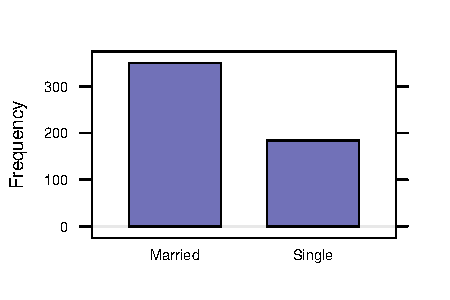
\includegraphics[width=.9\textwidth]{figures/fig-unnamed-chunk-23-1} 

}



\end{knitrout}

\subsubsection{A Caution Regarding Prediction Intervals}
Prediction intervals are much more sensitive to the normality assumption
than confidence intervals are because the Central Limit Theorem does not 
help when we are thinking about individual observations (essentially samples of 
size 1).

\begin{problem}
	Use the output below to answer some questions about rainfall volume  and 
	runoff volume (both in $m^3$) for a particular stretch of a Texas highway.
\begin{knitrout}
\definecolor{shadecolor}{rgb}{0.969, 0.969, 0.969}\color{fgcolor}\begin{kframe}
\begin{verbatim}
## 
## Call:
## lm(formula = runoff ~ rainfall, data = TexasHighway)
## 
## Residuals:
##    Min     1Q Median     3Q    Max 
## -8.279 -4.424  1.205  3.145  8.261 
## 
## Coefficients:
##             Estimate Std. Error t value Pr(>|t|)
## (Intercept) -1.12830    2.36778  -0.477    0.642
## rainfall     0.82697    0.03652  22.642  7.9e-12
## 
## Residual standard error: 5.24 on 13 degrees of freedom
## Multiple R-squared:  0.9753,	Adjusted R-squared:  0.9734 
## F-statistic: 512.7 on 1 and 13 DF,  p-value: 7.896e-12
\end{verbatim}
\end{kframe}
\end{knitrout}
	\begin{enumerate}
		\item
			How many times were rainfall and runoff recorded?
		\item
			What is the equation for the least squares regression line?
		\item
			Report the slope together with its standard uncertainty.
		\item
			Give a 95\% confidence interval for the slope of this line.
		\item
			What does this slope tell you about runoff on this
			stretch of highway?
		\item
			What is $\hat\sigma$?
	\end{enumerate}
\end{problem}

\begin{solution}
	\begin{enumerate}
		\item
			The residual degrees of freedom is $13$, so there were $13 + 2 = 15$
			observations.
\item
	$\variable{runoff} = -1  + 0.83 \cdot \variable{rainfall}$
\item
	$0.83 \pm 0.04$
\item
\begin{knitrout}
\definecolor{shadecolor}{rgb}{0.969, 0.969, 0.969}\color{fgcolor}\begin{kframe}
\begin{alltt}
\hlkwd{confint}\hlstd{(rain.model,} \hlstr{"rainfall"}\hlstd{)}
\end{alltt}
\begin{verbatim}
##              2.5 %    97.5 %
## rainfall 0.7480677 0.9058786
\end{verbatim}
\end{kframe}
\end{knitrout}
	We can compute this from the information displayed:
\begin{knitrout}
\definecolor{shadecolor}{rgb}{0.969, 0.969, 0.969}\color{fgcolor}\begin{kframe}
\begin{alltt}
\hlstd{t.star} \hlkwb{<-} \hlkwd{qt}\hlstd{(} \hlnum{.975}\hlstd{,} \hlkwc{df}\hlstd{=}\hlnum{13} \hlstd{)} \hlcom{# 13 df listed for residual standard error}
\hlstd{t.star}
\end{alltt}
\begin{verbatim}
## [1] 2.160369
\end{verbatim}
\begin{alltt}
\hlstd{SE} \hlkwb{<-} \hlnum{0.0365}
\hlstd{ME} \hlkwb{<-} \hlstd{t.star} \hlopt{*} \hlstd{SE; SE}
\end{alltt}
\begin{verbatim}
## [1] 0.0365
\end{verbatim}
\begin{alltt}
\hlnum{0.8270} \hlopt{+} \hlkwd{c}\hlstd{(}\hlopt{-}\hlnum{1}\hlstd{,}\hlnum{1}\hlstd{)} \hlopt{*} \hlstd{ME}  \hlcom{# CI as an interval}
\end{alltt}
\begin{verbatim}
## [1] 0.7481465 0.9058535
\end{verbatim}
\end{kframe}
\end{knitrout}
We should round this using our rounding rules (treating the margin of error
like an uncertainty).
\item
	The slope tells us how much additional run-off there is per additional
	amount of rain that falls.  Since both are in the same units ($m^3$) and
	since the intercept is essentially 0, we can interpret this slope as a
	proportion.  Roughly 83\% of the rain water is being measured as runoff. 
\item
	$5.24$
	\end{enumerate}
\end{solution}

\begin{problem}
Data from a 1993 study to see how well lichens serve as an indicator for air pollution
are in the \dataframe{ex12.20} data set in the \pkg{Devore6} package.  In that paper,
a simple linear model was fit to see how the wet deposition of $\mathrm{NO}_{3}^{-}$
($g N/m^2$) related to the percentage dry weight of lichen.
\begin{enumerate}
	\item What are the least squares estimates for the intercept and slope of a line
		that can be used to estimate deposition
		from the amount of lichen?
	\item
		What is the estimated value of $\sigma$?
	\item
		Predict the amount of deposition if the dry weight of the 
		lichen is measured to be $0.7$.
	\item
		Give a 95\% confidence interval for the mean amount deposition among
		among samples with a dry weight of lichen measured to be $0.7\%$.
\end{enumerate}
\end{problem}

\begin{solution}
\begin{knitrout}
\definecolor{shadecolor}{rgb}{0.969, 0.969, 0.969}\color{fgcolor}\begin{kframe}
\begin{alltt}
\hlkwd{require}\hlstd{(Devore6)}
\hlstd{lichen.lm} \hlkwb{<-} \hlkwd{lm}\hlstd{(deposition} \hlopt{~} \hlstd{LichenN,} \hlkwc{data} \hlstd{= ex12.20)}
\hlcom{# a)}
\hlstd{lichen.lm}
\end{alltt}
\begin{verbatim}
## 
## Call:
## lm(formula = deposition ~ LichenN, data = ex12.20)
## 
## Coefficients:
## (Intercept)      LichenN  
##     -0.1423       0.7421
\end{verbatim}
\begin{alltt}
\hlkwd{coef}\hlstd{(lichen.lm)}  \hlcom{# this includes standard errors; could also use summary() }
\end{alltt}
\begin{verbatim}
## (Intercept)     LichenN 
##  -0.1422980   0.7421083
\end{verbatim}
\begin{alltt}
\hlcom{# b)}
\hlkwd{sigmaHat}\hlstd{(lichen.lm)}  \hlcom{# can also be read off of the summary() output}
\end{alltt}
\begin{verbatim}
## [1] 0.169261
\end{verbatim}
\begin{alltt}
\hlcom{# c)}
\hlstd{estimated.dep} \hlkwb{<-} \hlkwd{makeFun}\hlstd{(lichen.lm)}
\hlkwd{estimated.dep}\hlstd{(}\hlnum{0.7}\hlstd{)}
\end{alltt}
\begin{verbatim}
##         1 
## 0.3771778
\end{verbatim}
\begin{alltt}
\hlcom{# d)}
\hlkwd{estimated.dep}\hlstd{(}\hlnum{0.7}\hlstd{,} \hlkwc{interval} \hlstd{=} \hlstr{"confidence"}\hlstd{)}
\end{alltt}
\begin{verbatim}
##         fit       lwr       upr
## 1 0.3771778 0.2688428 0.4855128
\end{verbatim}
\end{kframe}
\end{knitrout}
\end{solution}

\begin{problem}
	The \dataframe{KidsFeet} data set contains variables giving the widths and lengths
	of feet of some grade school kids.
	\begin{enumerate}
		\item
			Perform our usual diagnostics to see whether there are any reasons
			to be concerned about using a simple linear model in this situation.
		\item Based on this data, what estimate would you give for the width of a 
			Billy's foot if Billy's foot is 24 cm long?  
			(Use a 95\% confidence level.)
		\item Based on this data, what estimate would you give for the average width of a 
			kids' feet that 24 cm long?
			(Use a 95\% confidence level.)
	\end{enumerate}
\end{problem}

\begin{solution}
\begin{knitrout}
\definecolor{shadecolor}{rgb}{0.969, 0.969, 0.969}\color{fgcolor}\begin{kframe}
\begin{alltt}
\hlstd{foot.model} \hlkwb{<-} \hlkwd{lm}\hlstd{(width} \hlopt{~} \hlstd{length,} \hlkwc{data} \hlstd{= KidsFeet)}
\hlkwd{plot}\hlstd{(foot.model,} \hlkwc{w} \hlstd{=} \hlnum{1}\hlstd{)}
\hlkwd{plot}\hlstd{(foot.model,} \hlkwc{w} \hlstd{=} \hlnum{2}\hlstd{)}
\end{alltt}
\end{kframe}

{\centering 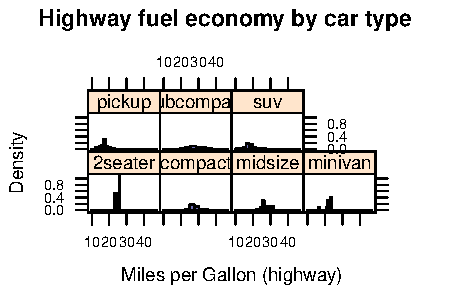
\includegraphics[width=\maxwidth]{figures/fig-unnamed-chunk-28-1} 
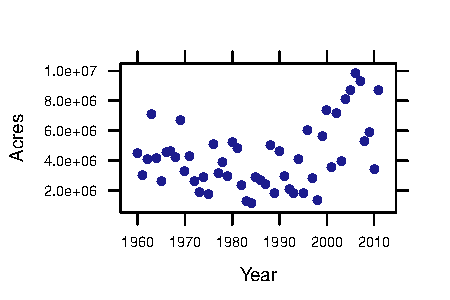
\includegraphics[width=\maxwidth]{figures/fig-unnamed-chunk-28-2} 

}



\end{knitrout}
Our diagnostics look pretty good.  The residuals look randomly distributed with
similar amounts of variability throughout the plot.  The normal-quantile plot
is nearly linear.

\begin{knitrout}
\definecolor{shadecolor}{rgb}{0.969, 0.969, 0.969}\color{fgcolor}\begin{kframe}
\begin{alltt}
\hlstd{f} \hlkwb{<-} \hlkwd{makeFun}\hlstd{(foot.model)}
\hlkwd{f}\hlstd{(}\hlnum{24}\hlstd{,} \hlkwc{interval} \hlstd{=} \hlstr{"prediction"}\hlstd{)}
\end{alltt}
\begin{verbatim}
##        fit      lwr      upr
## 1 8.813022 7.996604 9.629441
\end{verbatim}
\begin{alltt}
\hlkwd{f}\hlstd{(}\hlnum{24}\hlstd{,} \hlkwc{interval} \hlstd{=} \hlstr{"confidence"}\hlstd{)}
\end{alltt}
\begin{verbatim}
##        fit      lwr      upr
## 1 8.813022 8.665894 8.960151
\end{verbatim}
\end{kframe}
\end{knitrout}
We can't estimate Billy's foot width very accurately (between 8.0 and 9.6 cm),
but we can estimate the average foot width for all kids with a foot length of
24 cm more accurately (between 8.67 and 8.96 cm).
\end{solution}

\begin{problem}
	Some traffic engineers were interested to study interactions between bicycle and 
	automobile traffic.  One part of the study involved comparing the amount of 
	``available space'' for a bicyclist 
	(distance in feet from bicycle to centerline of the roadway) and 
	``separation distance'' 
	(the average distance between cyclists and passing car, also measured in feet, 
	determined by averaging based on photography over an extend period of time).
	Data were collected at 10 different sites with bicycle lanes.
	The data are available in the \dataframe{ex12.21} data set in 
	the \pkg{Devore6} package.

	\begin{enumerate}
		\item Write out an equation for the least squares regression line for 
			predicting separation distance from available space.
		\item Given an estimate (with uncertainty) for the slope and interpret it.
		\item A new bicycle lane is planned for a street that has 15 feet of available
			space.  Give an interval estimate for the separation distance 
			on this new street.  Should you use a confidence interval or a prediction
			interval?  Why?
		\item
			Give a scenario in which you would use the other kind of interval.
	\end{enumerate}
\end{problem}

\begin{solution}
\begin{knitrout}
\definecolor{shadecolor}{rgb}{0.969, 0.969, 0.969}\color{fgcolor}\begin{kframe}
\begin{alltt}
\hlstd{bike.model} \hlkwb{<-} \hlkwd{lm}\hlstd{(distance} \hlopt{~} \hlstd{space,} \hlkwc{data} \hlstd{= ex12.21)}
\hlkwd{coef}\hlstd{(}\hlkwd{summary}\hlstd{(bike.model))}
\end{alltt}
\begin{verbatim}
##               Estimate Std. Error   t value     Pr(>|t|)
## (Intercept) -2.1824715 1.05668813 -2.065388 7.274847e-02
## space        0.6603419 0.06747931  9.785841 9.974851e-06
\end{verbatim}
\begin{alltt}
\hlstd{f} \hlkwb{<-} \hlkwd{makeFun}\hlstd{(bike.model)}
\hlkwd{f}\hlstd{(}\hlnum{15}\hlstd{,} \hlkwc{interval} \hlstd{=} \hlstr{"prediction"}\hlstd{)}
\end{alltt}
\begin{verbatim}
##        fit      lwr      upr
## 1 7.722656 6.313278 9.132035
\end{verbatim}
\end{kframe}
\end{knitrout}
We would use a confidence interval to estimate the average separation distance 
for all streets with 15 feet of available space.
\begin{knitrout}
\definecolor{shadecolor}{rgb}{0.969, 0.969, 0.969}\color{fgcolor}\begin{kframe}
\begin{alltt}
\hlkwd{f}\hlstd{(}\hlnum{15}\hlstd{,} \hlkwc{interval} \hlstd{=} \hlstr{"confidence"}\hlstd{)}
\end{alltt}
\begin{verbatim}
##        fit      lwr      upr
## 1 7.722656 7.293168 8.152145
\end{verbatim}
\end{kframe}
\end{knitrout}
\end{solution}

\begin{problem}
	Select only the non-diabetic men from the \dataframe{pheno} data set using
\begin{knitrout}
\definecolor{shadecolor}{rgb}{0.969, 0.969, 0.969}\color{fgcolor}\begin{kframe}
\begin{alltt}
\hlkwd{require}\hlstd{(fastR)}  \hlcom{#pheno data are from the fastR package}
\hlstd{men} \hlkwb{<-} \hlkwd{subset}\hlstd{(pheno, sex} \hlopt{==} \hlstr{"M"} \hlopt{&} \hlstd{t2d} \hlopt{==} \hlstr{"control"}\hlstd{)}  \hlcom{# note the double == and quotes here}
\hlkwd{head}\hlstd{(men,} \hlnum{3}\hlstd{)}
\end{alltt}
\begin{verbatim}
##      id     t2d      bmi sex      age smoker chol waist weight height       whr sbp dbp
## 3  1012 control 30.47048   M 53.86161 former 5.02   104   94.6  176.2 0.9327354 143  89
## 20 1110 control 26.75386   M 68.07944  never 5.63    99   81.0  174.0 0.9252336 162  91
## 29 1146 control       NA   M 62.14521   <NA>   NA    NA     NA     NA        NA  NA  NA
\end{verbatim}
\end{kframe}
\end{knitrout}
This data set contains some phenotype information for subjects in
a large genetics study.  You can find out more about the data set with
\begin{knitrout}
\definecolor{shadecolor}{rgb}{0.969, 0.969, 0.969}\color{fgcolor}\begin{kframe}
\begin{alltt}
\hlopt{?}\hlstd{pheno}
\end{alltt}
\end{kframe}
\end{knitrout}
\begin{enumerate}
	\item
		Using this data, fit a linear model that can be used 
		to predict weight from height.  What is the equation 
		of the least squares regression line?
	\item
		Give a 95\% confidence interval for the slope of this regression
		and interpret it in context.  (Hint: what are the units?)
	\item
		Give a 95\% confidence interval for the mean weight of all 
		non-diabetic men who are 6 feet tall.  
		
		Note the heights are in cm and the weights are in kg, so you will need to convert 
		units to use inches and pounds.  (2.54 cm per inch, 2.2 pounds per kg)
	\item
		Perform regression diagnostics.  Is there any reason to be concerned
		about this analysis?
\end{enumerate}

\end{problem}

\begin{solution}
	\begin{enumerate}
		\item
\begin{knitrout}
\definecolor{shadecolor}{rgb}{0.969, 0.969, 0.969}\color{fgcolor}\begin{kframe}
\begin{alltt}
\hlstd{model} \hlkwb{<-} \hlkwd{lm}\hlstd{(weight} \hlopt{~} \hlstd{height,} \hlkwc{data} \hlstd{= men)}
\hlkwd{coef}\hlstd{(}\hlkwd{summary}\hlstd{(model))}
\end{alltt}
\begin{verbatim}
##                Estimate  Std. Error   t value     Pr(>|t|)
## (Intercept) -69.6988584 12.14450332 -5.739128 1.551023e-08
## height        0.8706793  0.06994051 12.448856 1.277243e-31
\end{verbatim}
\end{kframe}
\end{knitrout}
			So the equation is 
			\[
			\variable{weight} = 
			\ensuremath{-70} + 
			0.87 \cdot \variable{height}
			\]
		\item
\begin{knitrout}
\definecolor{shadecolor}{rgb}{0.969, 0.969, 0.969}\color{fgcolor}\begin{kframe}
\begin{alltt}
\hlcom{# we can ask for just the parameter we want, if we like}
\hlkwd{confint}\hlstd{(model,} \hlkwc{parm} \hlstd{=} \hlstr{"height"}\hlstd{)}
\end{alltt}
\begin{verbatim}
##            2.5 %   97.5 %
## height 0.7333052 1.008053
\end{verbatim}
\end{kframe}
\end{knitrout}
The slope tells us how much the average weight (in kg) increases per 
cm of height.
		\item
\begin{knitrout}
\definecolor{shadecolor}{rgb}{0.969, 0.969, 0.969}\color{fgcolor}\begin{kframe}
\begin{alltt}
\hlstd{f} \hlkwb{<-} \hlkwd{makeFun}\hlstd{(model)}
\hlcom{# in kg}
\hlkwd{f}\hlstd{(}\hlnum{6} \hlopt{*} \hlnum{12} \hlopt{*} \hlnum{2.54}\hlstd{,} \hlkwc{interval} \hlstd{=} \hlstr{"confidence"}\hlstd{)}
\end{alltt}
\begin{verbatim}
##        fit      lwr      upr
## 1 89.53098 87.97557 91.08639
\end{verbatim}
\begin{alltt}
\hlcom{# in pounds}
\hlkwd{f}\hlstd{(}\hlnum{6} \hlopt{*} \hlnum{12} \hlopt{*} \hlnum{2.54}\hlstd{,} \hlkwc{interval} \hlstd{=} \hlstr{"confidence"}\hlstd{)} \hlopt{*} \hlnum{2.2}
\end{alltt}
\begin{verbatim}
##        fit      lwr      upr
## 1 196.9682 193.5463 200.3901
\end{verbatim}
\end{kframe}
\end{knitrout}
		\item
\begin{knitrout}
\definecolor{shadecolor}{rgb}{0.969, 0.969, 0.969}\color{fgcolor}\begin{kframe}
\begin{alltt}
\hlkwd{xyplot}\hlstd{(}\hlkwd{resid}\hlstd{(model)} \hlopt{~} \hlkwd{fitted}\hlstd{(model))}
\hlkwd{qqmath}\hlstd{(}\hlopt{~}\hlkwd{resid}\hlstd{(model))}
\end{alltt}
\end{kframe}

{\centering 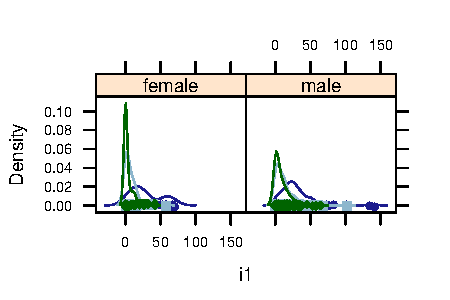
\includegraphics[width=\maxwidth]{figures/fig-unnamed-chunk-37-1} 
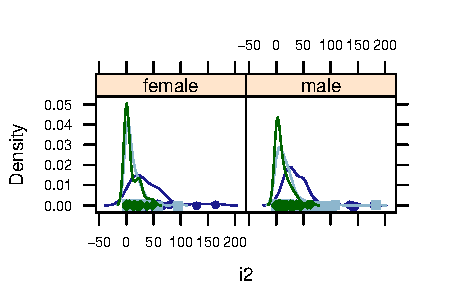
\includegraphics[width=\maxwidth]{figures/fig-unnamed-chunk-37-2} 

}



\end{knitrout}
We could also have used
\begin{knitrout}
\definecolor{shadecolor}{rgb}{0.969, 0.969, 0.969}\color{fgcolor}\begin{kframe}
\begin{alltt}
\hlkwd{plot}\hlstd{(model,} \hlkwc{which} \hlstd{=} \hlnum{1}\hlstd{)}
\hlkwd{plot}\hlstd{(model,} \hlkwc{which} \hlstd{=} \hlnum{2}\hlstd{)}
\end{alltt}
\end{kframe}

{\centering 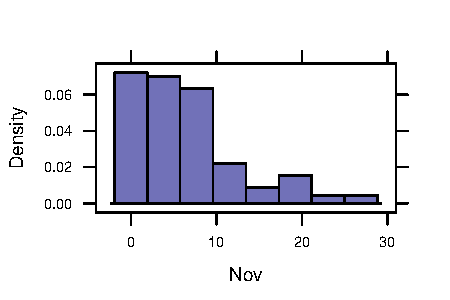
\includegraphics[width=\maxwidth]{figures/fig-unnamed-chunk-38-1} 
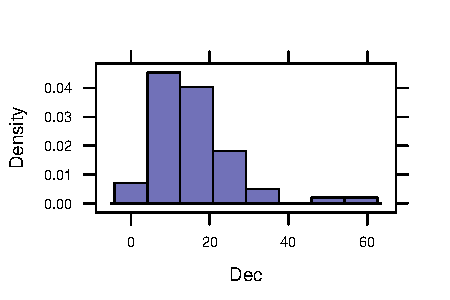
\includegraphics[width=\maxwidth]{figures/fig-unnamed-chunk-38-2} 

}



\end{knitrout}
The residual plot looks fine.  There is bit of a bend to the normal-quantile plot, indicating
that the distribution of residuals is a bit skewed (to the right -- the heaviest men are farther above
the mean weight for their height than the lightest men are below).

In this particular case, a log transformation of the weights improves the
residual distribution.  There is still one man whose weight is quite high for
his height, but otherwise things look quite good.
\begin{knitrout}
\definecolor{shadecolor}{rgb}{0.969, 0.969, 0.969}\color{fgcolor}\begin{kframe}
\begin{alltt}
\hlstd{model2} \hlkwb{<-} \hlkwd{lm}\hlstd{(}\hlkwd{log}\hlstd{(weight)} \hlopt{~} \hlstd{height,} \hlkwc{data} \hlstd{= men)}
\hlkwd{coef}\hlstd{(}\hlkwd{summary}\hlstd{(model2))}
\end{alltt}
\begin{verbatim}
##              Estimate   Std. Error  t value     Pr(>|t|)
## (Intercept) 2.5134829 0.1448876368 17.34781 2.145773e-54
## height      0.0108067 0.0008344117 12.95128 8.626095e-34
\end{verbatim}
\begin{alltt}
\hlkwd{xyplot}\hlstd{(}\hlkwd{resid}\hlstd{(model2)} \hlopt{~} \hlkwd{fitted}\hlstd{(model2))}
\hlkwd{qqmath}\hlstd{(}\hlopt{~}\hlkwd{resid}\hlstd{(model2))}
\end{alltt}
\end{kframe}

{\centering 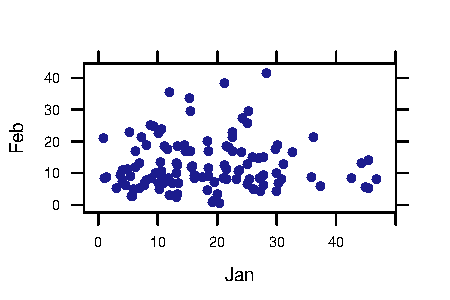
\includegraphics[width=\maxwidth]{figures/fig-unnamed-chunk-39-1} 
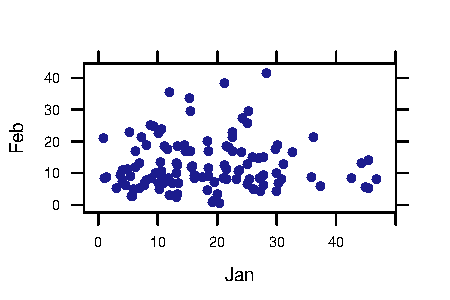
\includegraphics[width=\maxwidth]{figures/fig-unnamed-chunk-39-2} 

}



\end{knitrout}
This model says that
\[
\log( \variable{weight} ) 
	= 2.51 + 0.0108 \cdot \variable{height}
\]
So
\[
\variable{weight}  
= 12.3 
		\cdot (1.011)^{\variable{height}}
\]
\end{enumerate}
\end{solution}

\begin{problem}
	The \dataframe{anscombe} data set contains four pairs of explanatory 
	(\variable{x1}, \variable{x2}, \variable{x3}, and \variable{x4})
	and response
	(\variable{y1}, \variable{y2}, \variable{y3}, and \variable{y4})
	variables.  These data were constructed by Anscombe 
	\cite{Anscombe:1973:Graphs}.
	\begin{enumerate}
		\item 
			For each of the four pairs, us \R\ to fit a linear model and 
			compare the results.  Use, for example,
\begin{knitrout}
\definecolor{shadecolor}{rgb}{0.969, 0.969, 0.969}\color{fgcolor}\begin{kframe}
\begin{alltt}
\hlstd{model1} \hlkwb{<-} \hlkwd{lm}\hlstd{(y1} \hlopt{~} \hlstd{x1,} \hlkwc{data} \hlstd{= anscombe)}
\hlkwd{summary}\hlstd{(model1)}
\end{alltt}
\end{kframe}
\end{knitrout}
			Briefly describe what you notice looking at this output.  (You do not have
			to submit the output itself -- let's save some paper.)
		\item
			For each model, create a scatterplot that includes the regression line.
			(Make the plots fairly small and submit them.
			Use \texttt{fig.width} and \texttt{fig.height} to control the size of 
			the plots in RMarkdown.)
		\item
			Comment on the results.  Why do you think Anscombe invented these data?
	\end{enumerate}
\end{problem}

\begin{solution}
  Anscombe's data show that it is not sufficient to look only at the 
  numerical summaries produced by regression software.  His four data
  sets produce nearly identical output of \verb!lm()! and \verb!anova()!
  yet show very different fits.  An inspection of the residuals (or even
  simple scatterplots) quickly reveals the various difficulties.
\end{solution}

\begin{problem}
	Find an article from the engineering or science literature that uses 
	a simple linear model and report the following information:
	\begin{enumerate}
		\item
			Print the first page of the article (with title and abstract) and write
			a full citation for the article on it.  Staple this at the end of your
			assigment.
		\item
			If the article is available online, provide a URL where it can be found.
			(You can write that on the printout of the first page of the article, too.)
		\item
			How large was the data set used to fit the linear model?  How do you know?  (How 
			did the authors communicate this information?)
		\item
			What are the explanatory and response variables?
		\item
			Did the paper give an equation for the least squares regression line 
			(or the coefficients, from which you can determine the regression equation)?
			If so, report the equation
		\item
			Did the paper show a scatter plot of the data?  Was the regression line 
			shown on the plot?
		\item
			Did the paper provide confidence intervals or uncertainties for the 
			coefficients in the model?
		\item
			Did the paper show any diagnostic plots (normal-quantile, residuals plots, etc.)?
			If not, did the authors say anything in the text about checking that 
			a linear model is appropriate in their situation?
		\item
			What was the main conclusion of the analysis of the linear model?
		\item
				If there is an indication that the data are available online,
				let me know where in case we want to use these data for an example.
	\end{enumerate}
	Google scholar might be a useful tool for this.  JSTOR (available through Heckman
	Library) also has a large number of scientific articles.  Or you might ask an
	engineering or physics professor for an appropriate engineering journal to
	page through in the library.  Since the chances are small that two students
	will find the same article if working independently, I expect to see lots
	of different articles used for this problem.

	If your article looks particularly interesting or contains statistical 
	things that you don't understand but would like to understand, let me know,
	and perhaps we can do something later in the semester with your article.
	It's easiest to do this if you can give me a URL for locating the paper online.
\end{problem}


\newpage
\section*{Exercises}
\shipoutProblems


\ifsolutions
\ifsolutionslocal
\newpage
\section*{Solutions}
\shipoutSolutions
\fi
\fi

\bibliographystyle{amsalpha}
\bibliography{StatsBook,DataSets,jamstatassoc,RS,R,kaplan}
\end{document}
